%!TEX TS-program = pdflatex
\documentclass[10pt, a4paper, twoside]{article}
\usepackage{xltxtra} % for xelatex
\defaultfontfeatures{Ligatures=TeX}

\usepackage{hyperref}
\usepackage[
toc,
acronym,
nonumberlist,
style=altlist
]
{glossaries}
% renames must happen *before* babel package
\renewcommand{\glossaryname}{Stichwortverzeichnis}
\renewcommand{\acronymname}{Abkürzungsverzeichnis}
%Remove the dot at the end of glossary descriptions
\renewcommand*{\glspostdescription}{}

\usepackage[german,ngerman]{babel}

\usepackage{mflogo}
% \usepackage{amsmath}
% \usepackage{amssymb}
% \usepackage{pdfsync} % for use with Skim ctrl + cmd + w
\usepackage{graphicx}
\usepackage{url}
\usepackage{subfig}
\usepackage{wrapfig}
\usepackage{listings}
\usepackage{color}
\usepackage{xcolor}
\usepackage{courier} % for listings
\usepackage{fancyhdr}
\usepackage{tikz}
\usetikzlibrary{positioning} % for below, above, ...
\usetikzlibrary{trees} % for directory tree
\lstset{
	language=Ruby,
	basicstyle=\footnotesize\ttfamily,
	numbers=left,
	numberstyle=\tiny,
	tabsize=2,
	numbersep=7pt,
	xleftmargin=11pt,
	framexleftmargin=17pt,
	framexrightmargin=5pt,
	framexbottommargin=24pt,
	morekeywords={find,awk,printf,git},
	showspaces=false,
	showstringspaces=false
}
\DeclareCaptionFont{white}{\color{white}}
\DeclareCaptionFormat{listing}{\colorbox{gray}{\parbox{\textwidth}{#1#2#3}}}
\captionsetup[lstlisting]{format=listing,labelfont=white,textfont=white}
\usepackage[numbers]{natbib}
\bibliographystyle{natdin}

\newcommand{\entspricht}{\ensuremath{\mathrel{\widehat{=}}}}
\newcommand{\code}[1]{\texttt{\footnotesize{#1}}}
\newcommand{\HRule}{\rule{\linewidth}{0.5mm}}
\newcommand{\comment}[1]{}
\newcommand*\circled[1]{\tikz[baseline=(char.base)]{
  \node[shape=circle,draw,inner sep=1pt] (char) {#1};}}

\definecolor{grey}{rgb}{0.3,0.3,0.3}
\definecolor{lightgrey}{rgb}{0.8,0.8,0.8}

%-------------------------------------------
\pagestyle{fancy}
\fancyhf{} % delete current setting for header and footer

\setlength{\headheight}{17.5pt}
\fancyhead[RO]
{
  \bfseries\rightmark\quad~
  \colorbox{lightgrey}
  {
    \raisebox{0cm}[0.3cm][0.1cm]
    {
      \makebox[5cm][l]{\textbf{\thepage}}
    }
  }
  \hspace*{-6.5cm} % stupid but works
}
\fancyhead[LE]
{
  \hspace*{-6.5cm} % stupid but works
  {
    \colorbox{lightgrey}
    {
      \raisebox{0cm}[0.3cm][0.1cm]
      {
        \makebox[5cm][r]{\textbf{\thepage}}
      }
    } \quad~ \bfseries\leftmark
  }
}

% \fancyhead[LE,RO]{\bfseries\thepage}
% \fancyhead[LO]{\bfseries\rightmark}
% \fancyhead[RE]{\bfseries\leftmark}
 
\renewcommand{\headrulewidth}{0pt}
\renewcommand{\footrulewidth}{0pt}
\addtolength{\headheight}{0pt} % make space for the rule
%---------------------------------------------------------------------


\begin{document}
    
    \pagenumbering{Roman} % römische nummerierung für vorspiel
    
    \newglossaryentry{awk} {
  name=awk,
  description={ist eine musterorientierte Lese- und Verarbeitungssprache. Sie wird hier benutzt, um die Ausgabe eines \gls{find}-Befehls weiter zu verarbeiten. \cite{manpage_awk}}
}
\newglossaryentry{basecamp} {
  name=Basecamp,
  description={ist ein web-basiertes Projekt Management Tool der Firma 37signals. Damit können To-dos, Dateien, Nachrichten, Zeiten und Meilensteine verwaltet werden. (\url{http://basecamphq.com})}
}
\newglossaryentry{deployment} {
  name=Deployment,
  description={beschreibt alle Aktivitäten, eine Software in den Zustand zu überführen, in dem sie vom Endnutzer benutzt werden kann. Dazu gehören unter Anderem: Release, Installation, Aktivierung, Deaktivierung und Update. \cite{deployment_tech}}
}
\newglossaryentry{feature} {
  name=Feature,
  description={}
}
\newglossaryentry{feature_freeze} {
  name=Feature Freeze,
  description={(auch: Code Freeze) ist ein willkürlich definierter Zeitpunkt im Entwicklungszyklus einer Software, ab dem keine neuen Features mehr entwickelt werden. Bis zum nächsten Release wird ausschließlich an Stabilität gearbeitet. \cite[S.298]{praxiswissen_softwareing}}
}
\newglossaryentry{find} {
  name=find,
  description={ist ein UNIX-Werkzeug, um Dateien in einer Dateihierarchie zu finden. \cite{manpage_find}}
}
\newglossaryentry{git} {
  name=git,
  description={ist ein \gls{dvcs}. Es wurde von Linus Torvalds für die Linux Kernel Entwicklung geschrieben.}
}
\newglossaryentry{github} {
  name=GitHub,
  description={ist eine Hosting Plattform für \gls{git} Repositories. Es gibt sowohl öffentliche als auch private Repositories. Letztere sind für Firmen interessant, da diese ihre Projekte nicht für alle zugänglich haben wollen. Neben dem Hosting bietet die Plattform weitere Funktionalität wie Issue Tracking, News Feeds und grafische Auswertungen von Repositories. (\url{https://github.com/})}.
}
\newglossaryentry{inps} {
  name=inpsyde GmbH,
  description={ist eine deutsch Agentur, die sich auf das \gls{cms} \gls{wordpress} spezialisiert hat. (\url{http://inpsyde.com/})}
}
\newglossaryentry{jenkins} {
  name=Jenkins,
  description={(vorher: Hudson) ist eine in Java geschriebene Open Source \gls{ci} Software. (\url{http://jenkins-ci.org/})}
}
\newglossaryentry{json} {
  name=JSON,
  description={JavaScript Object Notation ist ein textbasiertes, sprachunabhängiges Datenaustauschformat. \cite{json}}
}
\newglossaryentry{mysql} {
  name=MySQL,
  description={ist ein von Oracle entwickeltes Datenbank Management System.}
}
\newglossaryentry{php} {
  name=PHP,
  description={ist eine populäre Scriptsprache zum Erstellen dynamischer Webseiten.}
}
\newglossaryentry{produktivsystem} {
  name=Produktivsystem,
  description={ist das öffentliche, dem Endnutzer verfügbare, System.}
}
\newglossaryentry{pull request} {
  name=Pull Request,
  description={ist Teil des Workflows bei der Arbeit mit dem Versionskontrollsystem git und der Plattform GitHub. Wird ein Feature in einem separaten Branch entwickelt, muss die Übernahme des Features durch einen Pull Request beantragt werden. Dieser beinhaltet alle Änderungen und kann sowohl akzeptiert als auch abgewiesen werden.}
}
\newglossaryentry{reposerver} {
  name=Repository-Server,
  description={ist ein Server, der Repositories verwaltet.}
}
\newglossaryentry{repository} {
  name=Repository,
  description={ist ein Ort, an dem Versionskontrollsysteme ihre Daten ablegen.}
}
\newglossaryentry{rsync} {
  name=rsync,
  description={ist ein Kommandozeilenwerkzeug zur Dateiübertragung.}
}
\newglossaryentry{ror} {
  name=Ruby on Rails,
  description={ist ein Open Source Full Stack Web Application Framework für die Programmiersprache Ruby.}
}
\newglossaryentry{ruby} {
  name=Ruby,
  description={ist eine objektorientierte Programmiersprache.}
}
\newglossaryentry{stagingsystem} {
  name=Stagingsystem,
  description={ist ein nicht öffentliches System. Es wird zur Qualitätssicherung verwendet. Um einen möglichst realistischen Eindruck vom Endprodukt zu bekommen, bildet das Stagingsystem die Konfiguration des Produktivsystems so gut wie möglich ab.}
}
\newglossaryentry{webhook} {
  name=Webhook,
  description={ist eine Möglichkeit, Daten zwischen Webservices über HTTP-Requests auszutauschen. Der empfangende Service E registriert eine URL beim sendenden Service S an, z.B. http://www.example.com/receive. Tritt ein Ereignis bei S ein, versendet S die Ereignisdaten an alle registrierten URLs.}
}
\newglossaryentry{wordpress} {
  name=WordPress,
  description={ist eine freie Open Source Blogging Software auf Basis von PHP und MySQL.}
}
\newglossaryentry{working directory} {
  name=Working Directory,
  description={ist Bestandteil des Versionskontrollsystems git. Es enthält die aktuellen Arbeitsdateien, an denen gerade gearbeitet wird.}
}
\newglossaryentry{zielsystem} {
  name=Zielsystem,
  description={ist Ziel eines Deploymentvorgangs. Ist entweder das Staging- oder das Produktivsystem.}
}

\newacronym{ftp}{FTP}{File Transfer Protocol}
\newacronym{cli}{CLI}{Command Line Interface}
\newacronym{sftp}{SFTP}{SSH File Transfer Protocol}
\newacronym{ssh}{SSH}{Secure Shell}
\newacronym{qa}{QA}{Quality Assurance}
\newacronym{ape}{APE}{Automatic Push Environment}
\newacronym{cms}{CMS}{Content Management System}
\newacronym{ci}{CI}{Continuous Integration}
\newacronym{ide}{IDE}{Integrated Development Environment}
\newacronym{dvcs}{DVCS}{Distributed Version Control System}
\newacronym{rest}{REST}{Representational state transfer}

\makeglossaries
	\begin{titlepage}

  \begin{center}

    % Nummerierung auf Titelseite entfernen
    \thispagestyle{empty} 

    % HTWK Logo
    
\includegraphics[height=25mm]{assets/HTWK.eps}

    \textsc{\LARGE HOCHSCHULE FÜR TECHNIK, WIRTSCHAFT UND KULTUR LEIPZIG}\\[1cm]

    \textsc{\LARGE \color{grey} Netzwerk- und Systemmanagement Semesterarbeit}\\[1cm]

    % Titel
    \HRule \\[0.4cm]
      {
        \huge \bfseries APE \\[0.4cm]
        \large Ein Service zur Deployment-Automatisierung mit Hilfe von Git
      }\\[0.4cm]
    \HRule \\[1.5cm]

    % Sonstige Angaben
    \begin{minipage}{0.85\textwidth}
      \begin{flushleft}
        \color{grey}
        \begin{description}
          \item [Autor]         \hfill Eric Teubert
          \item [E-Mail]        \hfill ericteubert@googlemail.com
          \item [Matrikel-Nr.]  \hfill 55343
          \item [Bewertung]     \hfill Prof. Dr. Klaus Hänßgen
        \end{description}
      \end{flushleft}
    \end{minipage}

    % Datum ganz unten
    \vfill
    {\large \today}

  \end{center}
\end{titlepage}
    \clearpage{\pagestyle{empty}\cleardoublepage}

\setcounter{tocdepth}{3}
\tableofcontents
\newpage
\listoffigures
\lstlistoflistings
\clearpage

%TODO beim reinnehmen dran denken cleardoublepage zu togglen!
%\begin{abstract}
%  Test
%\end{abstract}
%\thispagestyle{empty}
%\clearpage

\thispagestyle{empty}
\subsection*{Eidesstattliche Erklärung}
Ich erkläre hiermit an Eides statt, dass ich die vorliegende Arbeit
selbständig und ohne Benutzung anderer als der angegebenen Hilfsmittel
angefertigt habe. Die aus fremden Quellen (einschließlich elektronischer
Quellen) direkt oder indirekt übernommenen Gedanken sind ausnahmslos als
solche kenntlich gemacht.

\vspace{2cm}

\noindent Eric Teubert

% \clearpage
\clearpage{\pagestyle{empty}\cleardoublepage}

    \pagenumbering{arabic} % arabische nummerierung für hauptteil
    
    \section{Einleitung} % (fold)
\label{sec:einleitung}

Das Projekt entsteht im Auftrag der Agentur \gls{inps}. Diese erhofft sich Kosteinersparnis durch Automatisierung, sowie eine solidere rechtliche Basis gegenüber ihren Kunden.

Automatisierung wird an verschiedenen Stellen eingeführt. Da bereits das Versionskontrollsystem git verwendet wird, werden dessein Eigenschaften ausgenutzt. Hält ein Entwickler ein Feature für abgeschlossen, stellt er über den Service GitHub einen so genannten Pull Request. Alle am Projekt beteiligten Entwickler werden benachrichtigt und können Anmerkungen und sogar Änderungen vornehmen, bevor das Feature gemerged wird. Dies geschieht automatisch. Außerdem wird im Projektmanagement-Tool Basecamp eine zum Pull Request passende ToDo erstellt. Der Kunde wird außerdem per E-Mail benachrichtigt.

Letztgenannter Part ist insbesondere rechtlich interessant. Der Kunde kann das Feature nun in einer separaten Testumgebung ansehen und eventuell von seiner eigenen \gls{qa}-Abteilung verifizieren lassen. Ist der Kunde zufrieden, hakt er die ToDo ab und gibt damit sein Einverständnis. Es kann vertraglich geregelt werden, dass der Kunde sich der Qualität des Features versichert hat und somit die \gls{inps} keinerlei Kosten für eventuell auf diesem Feature basierenden Ausfällen übernimmt.

Die Bestätigung des Kunden löst einen weiteren Automatisierungsmechanismus auf. Das Feature wird in den produktiven Versionierungszweig gemerged und sofort auf das \gls{produktivsystem} deployed. Der Entwickler muss nichts weiter unternehmen und der Kunde kann sein akzeptiertes Feature ohne Verzögerung betrachten.

Insgesamt wird ein Service entwickelt, welcher die bereits genutzten Systeme GitHub und Basecamp verbindet und einige Automatisierungen durchführt. Die Integration ist dabei transparent. Weder Kunde noch Entwickler sieht jemals eine grafische Oberfläche des Services. Beide Parteien profitieren jedoch von den Automatisierungen und Absicherungen, welche der Service bietet.

% section einleitung (end)

\section{Konzepte und Werkzeuge} % (fold) 8+ Seiten, Allgemeines Kapitel
\label{sec:konzepte_und_werkzeuge}

Dieses Kapitel widmet sich den Grundlagen, die zum Verständnis der nachfolgenden Arbeit notwendig sind. Der Leser möge selbst entscheiden, wie vertraut er mit der jeweiligen Thematik bereits ist und bei Bedarf lediglich querlesen oder ganz überspringen.

\subsection{Konzepte} % (fold)
\label{sub:konzepte}

\gls{ape} ist ein Deployment-System. Dieses Kapitel erklärt, was das ist und welche Teilaufgabe davon \gls{ape} übernommt.

\subsubsection{Deployment} % (fold)
\label{ssub:deployment}

Deployment ist ein englischsprachiger Begriff. \emph{to deploy} kann mit \emph{einsetzen} und \emph{anwenden} übersetzt werden.

Im Bereich der Softwareentwicklung beschreibt es den Vorgang, ein entwickeltes Projekt oder Teilprojekt in einen Zustand zu überführen, so dass es vom Endbenutzer eingesetzt werden kann.

Arbeitet ein Entwickler an einem Projekt, so geschieht dies unter Idealbedingungen. Er hat seine lokalen Werkzeuge zur Verfügung und kann seine Arbeitsumgebung so konfigurieren, dass das Projekt am besten funktioniert. Diese Bedingungen unterscheiden sich jedoch vom \gls{produktivsystem}. Diese Tatsache muss beim Deployment beachtet werden.

Wird in Sprachen entwickelt, welche kompiliert werden müssen, entstehen zusätzliche Schwierigkeiten. Der korrekte Compiler muss in der korrekten Version verwendet werden. Während der Entwickler in der Programmierphase den Compile-Button seiner \gls{ide} verwenden kann, steht diese Funktion dem Endbenutzer nicht zur Verfügung. Dieser ist auf eine ausführbare Datei angewiesen.

Im Rahmen dieser Arbeit werden jedoch ausschließlich Webprojekte besprochen. Diese werden dynamisch interpretiert, nicht compiliert. Damit entfällt die besprochene Hürde.

Webentwicklung erfordert, dass das Projektverzeichnis zum Zielsystem übertragen wird. Dies geschieht entweder manuell oder automatisiert. Letztgenanntes ist erstrebenswert. Der Grund dafür wird unter Anderem in Kapitel \ref{ssub:continuous_deployment} besprochen.

% subsubsection deployment (end)

\subsubsection{Continuous Deployment} % (fold)
\label{ssub:continuous_deployment}

Mit wachsender Projektgröße steigt der Aufwand des Deployments. Außerdem besteht immer die Gefahr, dass beim Einspielen einer neuen Versions in das \gls{produktivsystem} Fehler entstehen. Je größer die Änderungen, desto höher ist die Wahrscheinlichkeit der Einführung neuer Fehler\comment{externe ref}. Continuous Deployment versucht, diese Probleme zu lösen oder zumindest einzugrenzen.

\emph{Continuous}, englisch \emph{kontinuierlich}, \emph{ständig} oder \emph{stetig}, beschreibt einen wesentlichen Aspekt. Es ist üblich, in Releases zu denken. Das heißt, es wird für Wochen oder Monate im Voraus geplant, woran gearbeitet wird. Erst, wenn dieser Plan abgearbeitet wurde, werden alle Änderungen zugleich deployed. Dies ist im Bereich des Webs aber weder erforderlich noch wünschenswert.

Es gibt mehrere Gründe, diesen Ansatz zu vermeiden. Zum einen steigt, wie bereits erwähnt, mit der Größe der Änderungen auch die Wahrscheinlichkeit eines Fehlers. Zum anderen muss Releasemanagement betrieben werden, um kritische Patches sowohl im \gls{produktivsystem} als auch im gerade entwickelten Release einfließen zu lassen. Weiterhin ist es im Sinne des Endkunden, wenn dieser schneller von neuen Features profitiert. Schließlich ist es um so schwieriger, einen Fehler einer Änderung zuzuordnen, je mehr Änderungen mit einem Mal deployed werden.

Mit Continuous Deployment ist es möglich, täglich oder sogar mehrmals täglich kleine Änderungen zu veröffentlichen. Kritische Patches können sofort im normalen Entwicklungsprozess behandelt werden. Endbenutzer profitieren sofort von Features. Auftretende Fehler können leichter der soeben eingeführten Änderung zugeordnet werden.

Dies ist jedoch nur realisierbar, wenn der Aufwand des Deployments klein ist. Das heißt, es soll so viel wie möglich automatisiert werden. Je weniger der Entwickler eingreifen muss, desto mehr Zeit kann er mit der Entwicklung von Features verbringen. Ist der Aufwand des Deployments zu groß, wird der Entwickler verleitet, mehrere Features zu einem Release zusammenzufassen, was dem Grundgedanken des Continuous Deployments widerspricht. Es handelt sich hierbei um eine psychologische Schranke. Mit anderen Worten, es ist für jeden Entwickler eine andere Interpretation von \emph{zu groß} notwendig. Schließlich kann nur das Ziel verfolgt werden, den Aufwand immer weiter zu verringern.

Angenommen, es existiert ein Deployment-System mit genügend geringem Aufwand, so dass kein Entwickler dazu tendiert, das System zu umgehen. Dann ist es auch möglich, auf beliebig viele Systeme zu deployen. Das ermöglicht die Existenz eines \glspl{stagingsystem}. Dieses kann identisch zum \gls{produktivsystem} sein -- mit dem einzigen Unterschied, dass es für Endbenutzer nicht erreichbar ist. Dann kann eine Änderung zuerst dorthin deployed und unter realistischen Bedingungen getestet werden. So können Fehler bereits auf diesem System entdeckt und behoben werden, bevor das neue Feature das \gls{produktivsystem} erreicht.

Das wiederum erlaubt eine größere Flexibilität im Arbeitsablauf. Eine \gls{qa} Abteilung kann selbstständig ein Testverfahren entwickeln und dieses jedes Mal durchlaufen, wenn eine neue Änderung das \gls{stagingsystem} erreicht.

\gls{ape} kommt zum Einsatz, um Continuous Deployment zu ermöglichen. Deployment wird vollkommen automatisiert. Ein Projekt muss lediglich zu Beginn einmalig konfiguriert werden. Anschließend übernimmt \gls{ape} das Deployment. Wie das möglich ist, wird ab Kapitel \ref{sec:architektur_und_umsetzung} erläutert.

% subsubsection continuous_deployment (end)

% subsection konzepte (end)

\subsection{Werkzeuge} % (fold)
\label{sub:werkzeuge}

Nachfolgend werden einige Werkzeuge und Teile derer Funktionen erläutert, die zum Verständnis der Arbeit notwendig sind.

\subsubsection{SSH \& Asymmetrische Authentifizierung} % (fold)
\label{ssub:ssh_&_asymmetrische_authentifizierung}

Wie in Kapitel \ref{sub:architektur} gezeigt wird, müssen verschiedene Systeme miteinander kommunizieren. Diese Kommunikation muss sowohl automatisch, als auch sicher stattfinden.

An mehreren Stellen wird \gls{ssh} zum Einsatz kommen. Dieses Protokoll erfüllt die genannten Bedingungen. Die Kommunikation ist mächtig, da über das Protokoll Shell-Befehle ausgeführt werden können. Die Authentifizierung kann durch die Verwendung eines asymmetrischen Schlüsselpaars automatisiert werden. Bei einer passwortbasierten Authentifizierung muss das Passwort interaktiv eingegeben werden, was eine Automatisierung verhindert. Asymmetrische Automatisierung gilt weiterhin als sicher.\comment{externe referenz}

% subsubsection ssh_&_asymmetrische_authentifizierung (end)

\subsubsection{git} % (fold)
\label{ssub:git}

Ein zentrales Werkzeug des Workflows ist \gls{git}. Es wird zur dezentralen Versionskontrolle verwendet. Im Zusammenspiel mit \gls{github} bildet es die Basis des Workflows.

Zum Verständnis der weiteren Arbeit ist es notwendig, einige grundlegende Kommandozeilenbefehle zu verstehen. Diese werden nun erklärt.

\paragraph{\lstinline!git clone <repository>!} % (fold)
\label{par:git_clone}
Klont ein \gls{repository} in ein lokales Verzeichnis. Dabei wird die Referenz zum Ursprungsrepository behalten, so dass dieses nicht bei jedem weiteren Befehl angegeben werden muss. Um es dennoch referenzieren zu können, bekommt es den Namen \lstinline!origin! und kann bei Bedarf damit angesprochen werden.
% paragraph git_clone (end)

\paragraph{\lstinline!git pull!} % (fold)
\label{par:git_pull}
Holt alle Änderungen aus dem \gls{repository} (im Rahmen dieser Arbeit ausschließlich \gls{github}).
% paragraph git_pull (end)

\paragraph{\lstinline!git push!} % (fold)
\label{par:git_push}
Sendet Änderungen aller lokalen Branches mit korrespondierendem entfernten Branch zum entsprechenden \gls{repository} (im Rahmen dieser Arbeit ausschließlich \gls{github}).
% paragraph git_push (end)

\paragraph{\lstinline!git checkout [-b] <branch>!} % (fold)
\label{par:git_checkout}
Holt einen Branch in das \gls{working directory}. Mit anderen Worten, es wird der angegebene Branch aktiviert und damit der Projektstatus dieses Branches hergestellt.

Wird der Parameter \lstinline!-b! verwendet, passieren zwei Dinge. Zuerst wird ein Branch des angegebenen Namens erstellt. Anschließend wird dieser ausgecheckt. In Kapitel \ref{ssub:staging_und_produktiv_deployment} wird folgender Befehl benötigt: \lstinline!git checkout -b live origin/live!. Dabei bezeichnet \lstinline!live! den lokal zu erstellenden Branch und \lstinline!origin/live! den aus\-zu\-check\-en\-den Branch auf \gls{github}.

% paragraph git_checkout (end)

\paragraph{\lstinline!git status!} % (fold)
\label{par:git_status}
Zeigt den Status des aktuellen \glspl{working directory}.
% paragraph git_status (end)

% subsubsection git (end)

\subsubsection{rsync} % (fold)
\label{ssub:rsync}

Um Daten von einem lokalen zu einem entfernten System zu kopieren, kann rsync verwendet werden. Es unterstützt rekursive Datentransfers, sowie Authentifizierung über \gls{ssh}.

Rsync wird zum Einsatz kommen, um Projektverzeichnisse auf Zielsysteme zu kopieren. Dies ist jedoch nur möglich, wenn diese \gls{ssh}-Authentifizierung unterstützen. Als Alternative kommt \gls{ftp} (Kapitel \ref{ssub:ftp}) zum Einsatz.

% subsubsection rsync (end)

\subsubsection{FTP} % (fold)
\label{ssub:ftp}

\gls{ftp} kommt im Rahmen dieser Arbeit als Ausweichsoption für \gls{rsync} zum Einsatz. Es wird benutzt, um Projektverzeichnisse von einem lokalen System auf ein Zielsystem zu kopieren. Die Authentifizierung findet über einen Benutzernamen sowie ein Passwort statt. \gls{ftp} ist langsamer als \gls{rsync}, kommt also nur zum Einsatz, wenn \gls{rsync} nicht möglich ist.

% subsubsection ftp (end)

\subsubsection{Ruby \& Ruby on Rails} % (fold)
\label{ssub:ruby_ruby_on_rails}

\gls{ape} wird mit \gls{ror} entwickelt.

\gls{ror} ist ein Open Source Full-Stack Web Application Framework für die Programmiersprache Ruby. Full-Stack bedeutet, dass das Framework -- und damit der Programmierer -- Zugriff auf Informationen des Webservers hat, Datenbankabfragen senden kann und ein Templatingsystem mitbringt.

Das Framework wurde ursprünglich aus dem Projekt \gls{basecamp} extrahiert, welches in dieser Arbeit auch besprochen wird. Das ist jedoch ein zufälliges Zusammentreffen. \gls{ape} hätte auch in einem anderen Framework implementiert werden können. \gls{ror} wurde insbesondere auf Basis der vorhandenen Kenntnisse des Entwicklers ausgewählt.

% subsubsection ruby_ruby_on_rails (end)

\subsubsection{WordPress} % (fold)
\label{ssub:wordpress}

\begin{wrapfigure}{l}{0.45\textwidth}
	\begin{tikzpicture}[%
		grow via three points={one child at (0.5,-0.7) and
		two children at (0.5,-0.7) and (0.5,-1.4)},
		edge from parent path={(\tikzparentnode.south) |- (\tikzchildnode.west)}]
		\tikzstyle{every node}=[anchor=west]
		\node {wp-content/}
		child { node {index.php}}		
		child { node {plugins/}
			child  { node {akismet/}}
			child  { node {bbPress/}}
		}
		child [missing] {}				
	    child [missing] {}
		child { node {themes/}
			child  { node {twentyeleven/}}
			child  { node {twentyten/}}
		}
		child [missing] {}				
	    child [missing] {}
		child { node {upgrade/}}
		child { node {uploads/}}
		;
	\end{tikzpicture}
	 \caption{Beispiel \lstinline!wp-content! Verzeichnis}
	 \label{fig:example_wp_content_dir}
\end{wrapfigure}

\gls{ape} wird darauf ausgelegt, \gls{wordpress}-Systeme zu deployen. Das heißt nicht, dass keine anderen Systeme damit verwaltet werden können. Da vorerst jedoch ausschließlich auf \gls{wordpress} basierende Projekte zum Einsatz kommen sollen, wird auch im Rahmen dieser Arbeit nichts anderes betrachtet.

\gls{wordpress} ist eine freie Open Source Blogging Plattform und \gls{cms} auf Basis von \gls{php} und \gls{mysql}. Unter anderem wegen seiner Plugin-Architektur und seinem Template-System eignet es sich, um verschiedenste Ansprüche erfüllen zu können.

Für das \gls{deployment} ist lediglich der Ordner \lstinline!wp-content! von Bedeutung. Alle außerhalb dieses Ordners liegenden Dateien gehören zu \gls{wordpress} selbst und sollten nie verändert werden, da sie nach einen \gls{wordpress} Update ohnehin wieder zurückgesetzt werden würden. Die einzige Ausnahme ist die Datei \lstinline!wp-config.php!, welche systembezogene Konfigurationen, wie Datenbank-Zugangsdaten, enthält.

Themes sind Dateien, welche Design und Funktionalität einer \gls{wordpress} Seite definieren. Plugins können unabhängig vom Theme eine Seite um Funktionalität erweitern oder bestehende Features verändern.

Veränderungen an der Datenbank werden von den Plugins und Themes selbst administriert. Das ist vorteilhaft, da das \gls{deployment} sich dann nicht darum kümmern muss. Es ist ausreichend, das \lstinline!wp-content! Verzeichnis zu aktualisieren.

% subsubsection wordpress (end)

% subsection werkzeuge (end)

% section konzepte_und_werkzeuge (end)

\section{Architektur und Umsetzung} % (fold) 10+ Seiten
\label{sec:architektur_und_umsetzung}

Das folgende Kapitel behandelt die Details des entstandenen Services. Zunächst wird erläutert, welches Problem \gls{ape} löst und weshalb genau dieser und kein anderer Ansatz gewählt wird. Anschließend werden Konzept und Architektur des Services analysiert, sowie einzelne Kernelemente der Software im Detail besprochen.

\subsection{Ziel des Services} % (fold)
\label{sub:ziel_des_services}

%% Welches Problem wird gelöst
\gls{ape} wird speziell für die Firma \gls{inps} entwickelt. Daher ist es zum Verständnis des Problems notwendig, eine Vorstellung von deren Dienstleistungen und Arbeitsabläufen zu haben.

\subsubsection{\gls{inps}} % (fold)
\label{ssub:inps}

Die \gls{inps} ist eine deutsche \gls{wordpress}-Agentur. Sie nimmt Aufträge von Kunden aller Größe an, um ihre Webseitenwünsche im \gls{cms} \gls{wordpress} umzusetzen. Die Auftragsbreite reicht von kleinen Pluginentwicklungen bis hin zur Konzeption und Umsetzung ganzer Blognetzwerke und Shopsysteme.

Ihre Mitarbeiter befinden sich verteilt in Mitteleuropa und arbeiten vorwiegend von zuhause. Damit arbeitet die \gls{inps} dezentral. Um je nach Auftragslage flexibel handeln zu können, werden mehr freie als fest angestellte Mitarbeiter beschäftigt.

An den kleinsten Projekten arbeiten einzelne Mitarbeiter, aber an der Mehrheit der Projekte arbeiten zwei oder mehr. Es gibt Projektleiter, welche Arbeit an die Entwickler verteilen und den größtmöglichen Teil der Kommunikation mit den Kunden übernehmen, damit die Entwickler ungestört arbeiten können. Dies sind die wesentlichen Rollen im Arbeitsfluss: Projektleiter, Entwickler und Kunde.

Der optimale Informationsfluss (Abbildung~\ref{fig:ideale-beziehung}) ist jedoch unrealistisch. Spätestens wenn das Projekt in Betrieb ist und Fehler berichtet werden, ist die Projektleiter-Schicht zum Teil eine unnötige Barriere. Um dennoch zu gewährleisten, dass der Kunde den Entwickler nicht direkt mit E-Mails oder Anrufen stört, wird das Projekt-Management Tool \Gls{basecamp} benutzt. Dort werden Fehlerberichte, sowie Featureanfragen in To-do-Listen verwaltet (Abbildung~\ref{fig:tatsaechliche-beziehung}).

Im Folgenden wird nicht mehr zwischen Fehlerbericht und Featureanfrage unterschieden werden. Aus Sicht des Arbeitsablaufs gibt es keinen Unterschied, daher ist es unnötig, beide Fälle zu betrachten. Es wird nur noch von Features die Rede sein.

\begin{figure}
	\centering
	\subfloat[Optimal] {
		\label{fig:ideale-beziehung}
		\begin{tikzpicture}%[scale=1.0,transform shape]
			\node (pm) {Projektleiter};
			\node (customer) [below=of pm] {Kunde}
				edge [<->] (pm)
			;
			\node (dev) [above=of pm] {Entwickler}
				edge [<->] (pm)
			;
		\end{tikzpicture}
	}
	\subfloat[Tatsächlich] {
		\label{fig:tatsaechliche-beziehung}
		\begin{tikzpicture}%[scale=1.0,transform shape]
			\node (center) {};
			\node (customer)	[left=of center]	{Kunde};
			\node (dev) 		[right=of center]	{Entwickler};
			\node (bc)			[above=of center]	{Basecamp}
				edge [<->,bend right] (customer)
				edge [<->,bend left] (dev)
			;
			\node (pm)			[below=of center]	{Projektleiter}
				edge [<->,bend left] (customer)
				edge [<->,bend right] (dev)
			;
		\end{tikzpicture}
	}
	
	\caption{Optimaler und tatsächlicher Informationsfluss}
	\label{fig:personen_beziehungen}
\end{figure}

% \begin{figure}
% 	\centering
% 	\begin{tikzpicture}[auto]
% 		\node (pm) {Projektleiter};
% 		\node (customer) [left=of pm] {Kunde}
% 			edge [<->] (pm)
% 		;
% 		\node (dev) [right=of pm] {Entwickler}
% 			edge [<->] (pm)
% 		;
% 	\end{tikzpicture}
% 	\caption{Optimaler Informationsfluss}
% 	\label{fig:ideale-beziehung}
% \end{figure}
% 
% \begin{figure}
% 	\centering
% 	\begin{tikzpicture}[auto]
% 		\node (center) {};
% 		\node (customer)	[left=of center]	{Kunde};
% 		\node (dev) 		[right=of center]	{Entwickler};
% 		\node (bc)			[above=of center]	{Basecamp}
% 			edge [<->,bend right] (customer)
% 			edge [<->,bend left] (dev)
% 		;
% 		\node (pm)			[below=of center]	{Projektleiter}
% 			edge [<->,bend left] (customer)
% 			edge [<->,bend right] (dev)
% 		;
% 	\end{tikzpicture}
% 	\caption{Tatsächlicher Informationsfluss}
% 	\label{fig:tatsaechliche-beziehung}
% \end{figure}

% subsubsection inps (end)

\subsubsection{Entwicklung eines Features} % (fold)
\label{ssub:entwicklung_eines_features}

Abhängig vom Projekt unterscheiden gibt es Abweichungen vom Arbeitsablauf. Doch die prinzipielle Vorgehensweise ist immer die gleiche. Diese wird nun beschrieben.

Der Kunde formuliert die Spezifikation für ein Feature oder eine Menge von Features. Diese werden vom Projekleiter begutachtet und eventuelle Unklarheiten werden im Dialog mit dem Kunden beseitigt. Ist das Projekt bereits fortgeschritten, formuliert der Kunde seine Wünsche direkt im Basecamp. Erfahrungsgemäß sind dies dann nur noch Anpassungen und Fehlerberichte, so dass der Projektleiter nicht mehr jede Anfrage kontrollieren muss.

Ein Entwickler weist sich eigenverantwortlich eine Teilaufgabe zu und beginnt, diese zu bearbeiten. Dazu stellt er sicher, dass er lokal die aktuelle Variante des Projekts vorliegen hat und beginnt, das Feature umzusetzen. Im Moment ist es dem Entwickler überlassen, ob er in separaten Branches arbeitet oder nicht. Sind mehrere Entwickler an einem Projekt beteiligt, sollen diese sich lediglich auf eine Vorgehensweise einigen.

Ist das Feature fertig entwickelt, werden die Änderungen manuell in ein Testsystem übertragen und der Kunde benachrichtigt. Der Kommunikationskanal ist dabei wieder projektabhängig. Ist der Kunde zufrieden, muss das Feature manuell auf das \gls{produktivsystem} übertragen werden.

Da der Vorgang insgesamt sehr aufwändig ist, wird vorwiegend in Releases gearbeitet. Das heißt, dass einige Tage oder Wochen Features entwickelt und in unregelmäßigen Abständen auf das Testsystem übertragen werden. An einem definierten Datum gibt es einen \gls{feature_freeze}. Einen Tag lang wird nur noch an der Stabilität des Releases gearbeitet und der Release selbst vorbereitet und durchgeführt. Verläuft dieser erfolgreich, beginnt der Zyklus erneut.

Diese Vorgehensweise funktioniert, ist jedoch umständlicher als sie sein müsste. Die Webplattform ist prädestiniert für tägliche oder mehrmals tägliche Releases. Es muss lediglich ein passender Workflow gefunden werden.

Weiterhin besteht im Moment das Problem, dass zwischen Projekten Unterschiede herrschen, die zwar klein aber doch vorhanden sind. Das sorgt dafür, dass Entwickler nicht konfliktfrei zwischen Projekten wechseln können. Es ist immer mit Verwirrung und Absprachen verbunden, die bei geeigneten Konventionen nicht nötig wären.

Dieses Problem soll \gls{ape} lösen. Es ist ein Workflow zu entferfen, welcher Konventionen einführt, der die oben genannten Abläufe vereinheitlicht. Automatisierungen sind, wo möglich, mit Hilfe der Software umzusetzen.

% subsubsection entwicklung_eines_features (end)

\subsection{Einheitlicher Workflow} % (fold)
\label{sub:einheitlicher_workflow}

Zunächst wird festgelegt, dass jedes Feature in seinem eigenen \gls{git}-Branch entwickelt wird. Das hat mehrere Vorteile. Entwickler in einem Projekt müssen sich weniger absprechen, da jeder in seinem eigenen Branch arbeitet. Ein Entwickler kann bei Prioritätenverschiebung zudem sofort die Arbeit an einem Feature anhalten und in einem parallelen Branch das wichtigere Feature bearbeiten. Auf Codeebene lässt sich mit einem einzigen \gls{git}-Befehl ermitteln, welche Zeilen das Feature verändert.

Weiterhin werden \gls{github} \glspl{pull request} ein fester Bestandteil des Workflows. Dies sind automatisierte Anträge, einen Branch in einen anderen zu mergen. Ein \gls{pull request} zeigt die Versionshistorie des Features und die Summe aller Änderungen. Andere Entwickler können das Feature reviewen, Anmerkungen hinterlassen und selbst Änderungen am Feature vornehmen. Sind alle Entwickler mit der Codequalität zufrieden, wird der \gls{pull request} akzeptiert und \gls{github} merged die Branches automatisch.

Es gibt zwei persistente \gls{git} Branches. \lstinline!dev! und \lstinline!live!. Letztgenannter ist unter allen Umständen stabil zu halten und wird darum nur in Ausnahmefällen manuell beeinflusst. Er ist ein Abbild des \gls{produktivsystem}s. Fertig entwickelte und vom Kunden bestätigte Features werden vom \gls{ape} in ihn gemerged. Analog dazu repräsentiert der \lstinline!dev! Branch das \gls{stagingsystem}. \gls{ape} merged Branches in \lstinline!dev!, wenn auf \gls{github} ein Pull Request akzeptiert wurde.

Ein \gls{pull request} wird vom Entwickler genau dann erstellt, wenn er mit der Entwicklung eines Features fertig ist und dieses bereit für das \gls{stagingsystem} ist. Wird dieser akzeptiert, sollen automatisch zwei Aktionen geschehen. Zum einen muss das Feature auf dem \gls{stagingsystem} verfügbar werden. Zum anderen soll der Kunde benachrichtigt werden, dass dieses Feature nun bereit zum testen ist. Beide Aufgaben werden vom \gls{ape} übernommen.

Der \gls{ape}-Service wird von GitHub per \Gls{webhook} informiert, dass ein Pull Request akzeptiert wurde. Zuerst wird das \gls{stagingsystem} aktualisiert. Dazu müssen lediglich die Dateien aus dem Staging-Branch übertragen werden, da \gls{github} bereits das Mergen der Branches übernommen hat. Anschließend wird über eine API in \gls{basecamp} ein To-do angelegt, welches den Kunden über das Feature im Testsystem informiert und um Feedback bittet. Basecamp verschickt automatisch eine E-Mail an den Kunden, so dass zwischen Akzeptanz des \glspl{pull request} und der automatischen Benachrichtigung des Kunden lediglich Sekunden oder Minuten liegen.

Gibt es Probleme, kann der Kunde diese über das Kommentarsystem in \gls{basecamp} äußern und der Entwickler kann diese bearbeiten. Ist der Kunde sofort oder nach Behebung aller Probleme zufrieden, kennzeichnet er dies durch das Abhaken der To-do. \gls{ape} registriert die Veränderung des Status der To-do automatisch und beginnt, das Feature auf das \gls{produktivsystem} zu übertragen. Dazu merged er selbstständig den Featurebranch in den Produktivbranch und überträgt das Ergebnis auf das \gls{produktivsystem}.

Damit ist ein Featurezyklus abgeschlossen. Ist das Feature klein (z.B. nur eine Codezeile muss angepasst werden) und reagieren alle Parteien schnell, kann der gesamte Zyklus einschließlich Programmierung in weniger als 15 Minuten abgearbeitet werden. Damit können selbst kritische Änderungen schnell vorgenommen werden. Es können beliebig viele dieser Zyklen parallel aktiv sein und ein Entwickler kann an verschiedenen Features gleichzeitig arbeiten, ohne dass sich deren Entwicklungsweige behindern.

% subsection einheitlicher_workflow (end)

\subsection{Architektur} % (fold)
\label{sub:architektur}

Das in dieser Arbeit betrachtete Gesamtsystem kann in sechs Komponenten unterteilt werden. Abbildung \ref{fig:ape_network} illustriert diese Unterteilung. Die sechs Komponenten sind: \circled{1} die Entwickler der \gls{inps}, \circled{2} \gls{github}, \circled{3} der \gls{ape}, \circled{4} die \gls{ape} Repositories, \circled{5} \gls{basecamp} und \circled{6} die Staging- und Produktivsysteme der Kunden.

\begin{figure}
	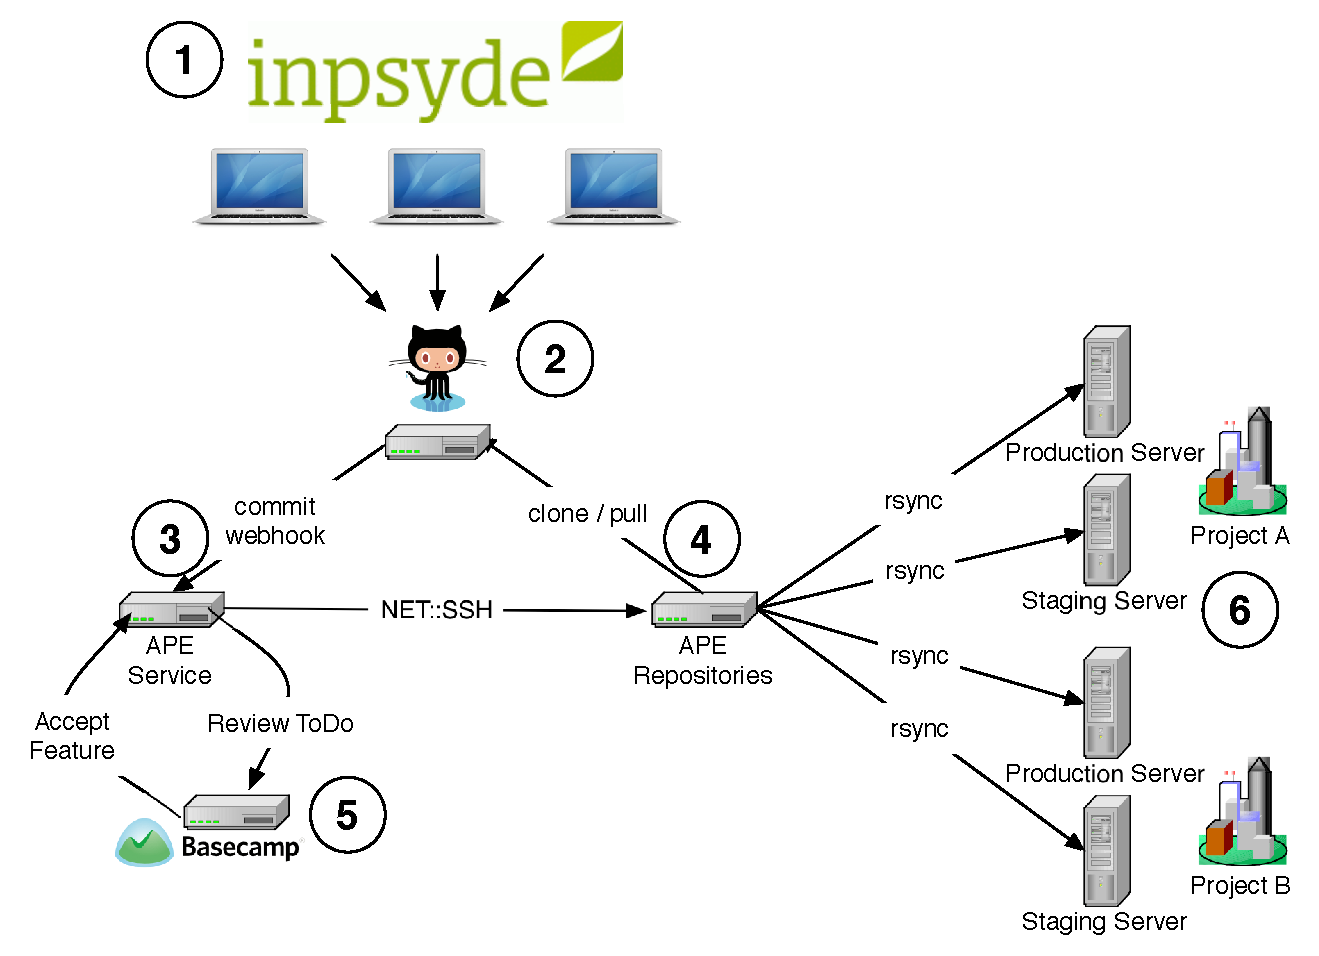
\includegraphics[width=1.0\textwidth]{assets/ape_network.eps}
	\caption{APE Netzwerk}
	\label{fig:ape_network}
\end{figure}

Zwischen den Entwicklern und \gls{github} gibt es zwei Schnittstellen. \gls{git} und die Webseite von \gls{github}: \url{https://github.com/}. \gls{git} kommt zur Verwaltung des Quellcodes zum Einsatz. Über die Webseite können die Entwickler miteinander kommunizieren und \glspl{pull request} erstellen.

\gls{github} sendet über eine Web-API automatisiert Informationen an \gls{ape}. Diese Schnittstelle kann über die \gls{github} Webseite konfiguriert werden.

\gls{basecamp} To-dos werden vom \gls{ape} erstellt. Dies geschieht über eine XML-basierte \gls{rest} API, welche von \gls{basecamp} bereitgestellt wird. Die Authentifizierung funktioniert über ein von \gls{basecamp} generiertes API Token.

Ein Server mit den \gls{ape} Repositories enthält die geklonten \lstinline!git! Repositories. Der Klonvorgang geschieht per direktem Zugriff auf \gls{github} über ein asymmetrisches Authentifizierungsverfahren. Dazu muss im jeweiligen \gls{github} Projekt der Public Key hinterlegt werden. Im Deployment-Vorgang loggt sich der \gls{ape} Service über SSH in die \gls{ape} Repositories ein. Auch dazu wird ein asymmetrisches Authentifizierungsverfahren verwendet.

Schließlich gibt es außerdem die Staging- und Produktivsysteme der Kunden. Je nach Projekt ein \gls{stagingsystem} für den Testbetrieb und ein \gls{produktivsystem} für die für die Welt sichtbare Webseite. Daten werden ausschließlich von den \gls{ape} Repositories zum entsprechenden Zielsystem transferiert. Dieser Transfer geschieht je nach Kundenwunsch entweder über \gls{ftp} oder \gls{rsync}.

Damit sind alle Komponenten betrachtet. Je nach Kunde kann es Abweichungen geben aber das Gesamtbild bleibt gleich. \gls{ape} Service und \gls{ape} Repositories könnten zum Beispiel auf dem selben System liegen. Aus Flexibilitätsgründen wurde jedoch die vorliegende Variante implementiert.

% subsection architektur (end)

\subsection{Alternativen} % (fold)
\label{sub:alternativen}

Es gibt beliebig viele Ansätze, die zu Anfang genannten Probleme zu lösen. Der soeben beschriebene Workflow ist einer davon. Weitere Herangehensweisen lassen sich unter anderem nach den Kriterien bewerten, wie viel Freiraum dem Entwickler gelassen wird, wie groß der Anteil der Automatisierung ist und wie viel manuell kommuniziert werden muss.

Die Wahl der Werkzeuge ist ausschließlich darin begründet, dass die \gls{inps} diese bereits erfolgreich im Einsatz hat und keinen Grund sieht, diese gegen neue einzutauschen. Es ist denkbar, ein einziges System zu entwickeln, welches die Features aller benötigten Services vereint. Doch der entstandene Mehrnutzen würde den ungleichmäßig höheren Aufwand nicht rechtfertigen.

Interessant wird die Idee des \gls{ape} insbesondere in Beziehung mit \gls{ci} Systemen. Eine häufig verwendete Open Source Anwendung ist \gls{jenkins}\footnote{http://jenkins-ci.org/}. Ist ein solcher Service bereits im Einsatz, bietet sich dieser als Plattform an, um die Konzepte hinter \gls{ape} umzusetzen, zum Beispiel über ein Plugin. Das erspart die Erstellung und Verwaltung einer vollständig neuen Plattform.
% subsection alternativen (end)

% subsection ziel_des_services (end)

\subsection{Implementierungsdetails} % (fold)
\label{sub:implementierungsdetails}

Für die Entwicklung des \gls{ape}-Services sind keine komplizierten Algorithmen notwendig. Die Schwierigkeit liegt im reibungslosen Verknüpfen der verschiedenen Services. Ein Schema der existierenden Schnittstellen ist in Abbildung\comment{fehlt} zu sehen. Im Folgenden werden einige ausgewählte nichttriviale Aspekte der Schnittstellenimplementierung besprochen.

\subsubsection{Interpretation von Git-Commits} % (fold)
\label{ssub:interpretation_von_git_commits}

Eine kritische Schnittstelle ist die Kommunikation zwischen \gls{github} und \gls{ape}. Jedes Mal, wenn ein Entwickler eine oder mehrere Änderungen über einen \lstinline!git push! zu \gls{github} transferiert, generiert \gls{github} bei Bedarf eine \gls{json}-formatierte Nachricht mit allen relevanten Informationen zum Repository, sowie zu den im \lstinline!push! enthaltenen Commits. Ein Beispieldatensatz ist in Listing \ref{lst:example_payload} zu sehen.

\begin{lstlisting}[caption=Beispiel-Webhook von \gls{github},label={lst:example_payload}]
{
  "before": "f7a3133afc170eebcc97349bae547558088a50cb",
  "repository": {
    "url": "http://github.com/inpsyde/ape",
    "name": "ape",
    "description": "Automatic Push Environment",
    "watchers": 5,
    "forks": 2,
    "private": 1,
    "owner": {
      "email": "e.teubert@inpsyde.com",
      "name": "eteubert"
    }
  },
  "commits": [
    {
      "id": "177e12cbcc29c84765f4232c87efb6a6c4cfb194",
      "url": "https://github.com/inpsyde/ape/commit/177e\
				12cbcc29c84765f4232c87efb6a6c4cfb194",
      "author": {
        "email": "e.teubert@inpsyde.com",
        "name": "Eric Teubert"
      },
      "message": "escape bash dollars",
      "timestamp": "2011-12-19T14:57:17-08:00",
      "added": ["ftp_tree.rb"]
    }
  ],
  "after": "177e12cbcc29c84765f4232c87efb6a6c4cfb194",
  "ref": "refs/heads/dev"
}
\end{lstlisting}

Diese Datensätze kann \gls{github} über einen so genannten Webhook an eine ausgewählte URL senden, zum Beispiel \lstinline!http://www.ape-service.com/github/webhook!. Mit Hilfe der \lstinline!repository!-Informationen wird das zu verwaltende Projekt bestimmt. Aus den Inhalten von \lstinline!ref! und \lstinline!commits! leitet \gls{ape} ab, welche Aktion auszuführen ist.

Aus \lstinline!ref! lässt sich der Branchname ableiten. Ist dieser weder \lstinline!dev! noch \lstinline!live!, wurde ein Feature entweder erstellt oder aktualisiert -- je nachdem, ob \gls{ape} das Feature bereits kennt oder nicht.

Ist \lstinline!dev! der abgeleitete Branchname, wurde ein Feature in diesen Branch gemerged und muss gestaged werden. Das Feature muss aus dem Inhalt des Commits abgeleitet werden. \gls{github} erzeugt bei akzeptierten Pull Requests Commit-Nachrichten der Form \lstinline!"Merge pull request #1 from <reponame>/<featurebranch>"!. Da diese Zeile immer gleich aufgebaut ist, lässt sich so zuverlässig der Featurebranch ermitteln.

Ähnlich verhält es sich, wenn \lstinline!live! der abgeleitete Branchname ist. Lediglich die Nachricht hat nun eine andere Form, da diese nicht durch einen Pull Request, sondern durch einen vom \gls{ape} durchgeführten \lstinline!git merge! generiert wird. Eine Nachricht hat die feste Struktur \lstinline!"Merge branch '<featurebranch>'"! und kann damit ohne Probleme geparsed werden. Schließlich wird der \lstinline!live! Branch auf das \gls{produktivsystem} deployed.

% subsubsection interpretation_von_git_commits (end)

\subsubsection{Staging und Produktiv-Deployment} % (fold)
\label{ssub:staging_und_produktiv_deployment}

Die Vorgänge beim Deployment unterscheiden sich kaum. Der Vorgang des Produktiv-Deployment, also das Deployen des \lstinline!live! Branches in das \gls{produktivsystem}, enthält einen zusätzlichen Schritt, daher wird dies als Beispiel herangezogen.

Zunächst öffnet \gls{ape} einen SSH Tunnel, um sich in den \gls{reposerver} einzuloggen. Dort wird, falls er noch nicht existiert, ein Ordner für das Projekt angelegt. Mit \lstinline!git status! wird anschließend überprüft, ob das Projekt bereits aus \gls{github} geklont wurde. Falls nicht, wird dies nun nachgeholt. Sollte dies fehlschlagen, gibt es ein Authentifizierungsproblem zwischen \gls{ape} und \gls{github}, welches behoben werden muss. Erst dann kann der Vorgang fortgesetzt werden.

Nachfolgend kann der \lstinline!live! Branch mit \lstinline!git checkout live! ausgecheckt werden. Schlägt dies fehl, bedeutet das, dass der Branch noch nie ausgecheckt wurde. Um dies nachzuholen, muss der Branch explizit erstellt und mit dem Branch auf \gls{github} verknüpft werden: \lstinline!git checkout -b live origin/live!. Schließlich kann der Branch mit \lstinline!git pull origin live! auf den aktuellen Stand gebracht werden. Eine Zusammenfassung des Vorgangs ist in Listing \ref{lst:git_checkout_live} zu sehen.

\begin{lstlisting}[caption=Wechsel auf den aktualisierten Deployment Branch,label={lst:git_checkout_live}]
out = ssh.exec_in_path!(path, "git checkout live")
if out =~ /error: pathspec 'live' did not match/
  ssh.exec_in_path!(path, "git checkout -b live origin/live")
end
ssh.exec_in_path!(path, "git pull origin live")
\end{lstlisting}

Anschließend muss der Featurebranch in \lstinline!live! gemerged werden -- aber nur, wenn das Deployment vom Kunden über \gls{basecamp} ausgelöst wurde. Sollte ein Entwickler direkt einen \gls{pull request} in den \lstinline!live! Branch unternommen haben, ist der Merge bereits geschehen. Treten beim Merge Konflikte auf, müssen zwei Dinge passieren. Zum einen wird der Merge mit \lstinline!git reset --hard live! zurückgenommen und der Deployment-Vorgang abgebrochen. Zum anderen wird ein Entwickler benachrichtigt, dass er selbst mergen und die Konflikte beheben muss.

An diesem Punkt angekommen, befindet sich auf dem \gls{reposerver} exakt der Projektstand, der deployed werden soll. Nun müssen diese Daten lediglich übertragen werden, um den Vorgang abzuschließen. Dieses komplexe Thema wird separat in Kapitel \ref{ssub:uebertragung_der_dateien} besprochen.

% subsubsection staging_und_produktiv_deployment (end)

\subsubsection{Übertragung der Dateien} % (fold)
\label{ssub:uebertragung_der_dateien}

Im Folgenden wird das Übertragen der Dateien vom Git-Repository zum Zielsystem beschrieben. Je nach Serversetup sind verschiedene Übertragungsmechanismen notwendig. Im Moment kann ein Produkt über \gls{ftp}, sowie \gls{ssh} deployed werden.

Die Anforderung besteht darin, Dateien zu übertragen. Dabei bestimmen verschiedene Faktoren über die Güte des verwendeten Verfahrens. Es wird vorausgesetzt, dass alle Dateien fehlerfrei übertragen werden. Ein Verfahren gilt als besser, wenn es dieses Ziel in kürzerer Zeit erreichen kann. Weiterhin sind Systeme vorzuziehen, welche den Ausschluss einzelner Verzeichnisse aus der Übertragung zulassen. Diejenigen, welche nur zur Entwicklung benötigt werden, müssen nicht auf Zielsysteme übertragen werden.

\paragraph{Deployment mit SSH} % (fold)
\label{par:deployment_mit_ssh}

Ein Zugang über \gls{ssh} setzt voraus, dass ein Schlüsselpaar generiert und eingerichtet ist. Ist diese Voraussetzung erfüllt, gibt es aufgrund der Mächtigkeit des Protokolls verschiedene Möglichkeiten, das Produkt tatsächlich zu übertragen.

Es wird davon ausgegangen, dass alle Produkte mit Git verwaltet werden. Daher ist es denkbar, sich auf das Zielsystem per \gls{ssh} einzuloggen und dort im \Gls{deployment}-Pfad mit einem \lstinline!git pull! das Produkt zu aktualisieren. Dies setzt jedoch voraus, dass das Programm git auf allen Zielsystemen installiert ist. Die Konfiguration der einzelnen Server ist aber ungewiss und kann nicht immer beeinflusst werden. Daher wird auf diesen Ansatz verzichtet.

Stattdessen wird das Produkt mit rsync\comment{externe referenz bietet sich an} übertragen. Rsync ist eine Anwendung, um Dateien und Verzeichnisse zwischen Servern zu synchronisieren. Durch die Verwendung von Delta Encoding\comment{externe referenz bietet sich an} ist der Vorgang zudem effizienter als bei einer normalen Dateiübertragung. Ein weiteres für diesen Anwendungsfall nützliches Feature ist die Möglichkeit, einzelne Verzeichnisse von der Übertragung auszuschließen. Auf den Zielsystemen wird nicht entwickelt, daher kann auf das .git Verzeichnis verzichtet werden. Ein Aufruf sieht beispielhaft wie folgt\comment{LaTeX-Referenz draus machen} aus:

> rsync -r --exclude=.git <lokaler-pfad> <user>@<host>:<entfernter-pfad>

Der Parameter \lstinline!-r! sorgt für eine rekursive Übertragung aller Verzeichnisse. Die Möglichkeit, über den \lstinline!--exclude! Parameter Verzeichnisse ausschließen zu können ist nicht notwendig, aber vorteilhaft. Das .git Verzeichnis beinhaltet tausende kleiner Dateien, welche den Übertragungsvorgang verlangsamen würden.

Insgesamt ist die Dateiübertragung mit rsync über \gls{ssh} zu bevorzugen. Mit dem einen oben genannten Befehl\comment{LaTeX-Referenz draus machen} werden alle Anforderungen erfüllt.

% paragraph deployment_mit_ssh (end)

\paragraph{Deployment mit FTP} % (fold)
\label{par:deployment_mit_ftp}

Aus verschiedenen Gründen kann es sein, dass eine Übertragung der Dateien über \textbf{SSH} nicht möglich ist. Als alternative Option wird das File Transfer Protocol \gls{ftp} angeboten. Im Folgenden werden zunächst die wesentlichen Einschränkungen und Nachteile des Protokolls formuliert.

Als erstes muss der Sicherheitsaspekt bedacht werden. Im Gegensatz zu \gls{ssh} geschieht die \gls{ftp}-Authentifizierung über Nutzername und Passwort. Da alle Vorgänge automatisiert stattfinden sollen, muss das \gls{ftp}-Passwort im Klartext in der Datenbank hinterlegt sein. Eine Verschlüsselung ist möglich, jedoch kein Hashing. Dieses wird sonst für Passwörter verwendet, um einen Rückschluss auf das Klartextpasswort zu verhindern. Darum muss darauf geachtet werden, dem \gls{ftp}-Nutzer nur die minimal nötigen Rechte einzuräumen.

Weiterhin verfügt das Protokoll nur über einen eingeschränkten Sprachschatz. Verzeichnisse können nicht rekursiv übertragen werden. Es können Dateien aus dem jeweils aktuellen Verzeichnis übertragen werden. Dabei ist es notwendig, dass sowohl lokal als auch auf dem Zielsystem in jedes Verzeichnis des Produkts gewechselt wird.

Da all das vollautomatisiert ablaufen muss, wurde ein Algorithmus entwickelt, welcher für ein gegebenes Projekt ein \gls{ftp}-Script zur Übertragung generiert. Zunächst wird mit Hilfe von find\comment{externe referenz bietet sich an} eine Liste aller Pfade ermittelt. Ein Beispiel ist in Listing \ref{lst:gen_path_list} zu sehen.

\begin{lstlisting}[caption=Generiere Liste aller Pfade,label={lst:gen_path_list}]
> find <path> -ls -path '*/.git*' -prune |\
	awk '{printf $3; for(x=11;x<=20;x++)\
	{printf " %s", $x} printf "\n" }'
\end{lstlisting}

Der \gls{find}\comment{externe referenz bietet sich an} Befehl schließt mit Hilfe der Parameter \lstinline!-path '*/.git*' -prune! das git Verzeichnis aus der Ergebnisliste aus. Außerdem wird mit \lstinline!-ls! eine detailliertere Ausgabe erzwungen, da die Information benötigt wird, ob ein gefundenes Objekt eine Datei oder ein Verzeichnis ist. Mit Hilfe von \gls{awk}\comment{externe referenz bietet sich an} wird die Ausgabe auf die Dateimodi, sowie den Pfad reduziert. Eine Beispielausgabe ist in Listing \ref{lst:gen_path_list_example} zu sehen.

\begin{lstlisting}[caption=Beispielausgabe für gefundene Pfade,label={lst:gen_path_list_example}]
	drwxr-xr-x ./bar
	-rw-r--r-- ./bar/baz.rb
	-rw-r--r-- ./bar/foo.rb
	-rw-r--r-- ./impress.md
	-rw-r--r-- ./index.php
	-rw-r--r-- ./README
\end{lstlisting}
     
Anschließend wird anhand dieser Ausgabe eine Baumdatenstruktur erstellt, welche das Verzeichnis repräsentiert. Nun kann mit Hilfe des Visitor-Patterns\comment{externe referenz bietet sich an} das \gls{ftp}-Script generiert werden. Trifft der Visitor auf eine Datei, wird diese mit \lstinline!put <datei>! übertragen. Der Pseudocode zum Verarbeiten eines Verzeichnisses ist in Listing \ref{lst:process_dir} zu sehen.

\begin{lstlisting}[caption=Verarbeitung eines Verzeichnisses,label={lst:process_dir}]
	out = Array.new
	out << "mkdir <verzeichnisname>
	out << "lcd <verzeichnisname>
	out << "cd <verzeichnisname>
	for all children { out << child.receive }
	out << "lcd .."
	out << "cd .."
	return out
\end{lstlisting}

Nachdem das Verzeichnis auf dem Zielsystem erstellt wurde, wird es sowohl lokal als auch im Ziel betreten. Anschließend werden rekursiv alle Kindknoten — also Dateien und eventuell weitere Verzeichnisse — abgearbeitet. Schließlich wird das Verzeichnis wieder verlassen.

% paragraph deployment_mit_ftp (end)

\paragraph{Vergleich der Deployment Varianten} % (fold)
\label{ssub:vergleich_der_deployment_varianten}

Während über \gls{ssh} ein einziger rsync-Befehl ausreicht, um alle Andforderungen zu erreichen, muss für \gls{ftp} ein ganz eigener Algorithmus implementiert werden. Die \gls{ssh}-Authentifizierung ist sicher, da sie über ein Schlüsselpaar hergestellt wird. \gls{ftp} hingegen ist auf ein Klartext-Passwort angewiesen. Außerdem ist rsync schneller und damit effizienter als \gls{ftp}\comment{externe referenz bietet sich an}. Wenn die Auswahl besteht, sollte daher immer die \gls{ssh}-Variante vorgezogen werden.

% paragraph vergleich_der_deployment_varianten (end)

% subsubsection Übertragung_der_dateien (end)

% subsection implementierungsdetails (end)

% section sec:architektur_und_umsetzung (end)

\section{Zusammenfassung und Ausblick} % (fold)
\label{sec:zusammenfassung_und_ausblick}
% - Was kann's? -> Highlights
% - Was wird in naher Zeit umgesetzt?
% - Was sind die Visionen?
% - evtl. Diskussion von Alternativen
% section zusammenfassung_und_ausblick (end)

    
	\printglossaries
	
    % \newpage
    % \bibliography{ape}
\end{document}